\section{Domain Analysis}

\subsection{Objective of the Laboratory Work}

The objective of this laboratory work is to port the bare-metal button press monitoring application developed in Lab~2.1 to a preemptive real-time operating system (FreeRTOS) running on the Arduino Mega 2560 microcontroller. The system retains the same functional requirements --- monitoring button press durations, providing visual LED feedback, and periodically reporting statistics over the STDIO serial interface --- but replaces the cooperative non-preemptive scheduler with FreeRTOS preemptive task management.

The key learning objectives include understanding preemptive scheduling in embedded real-time operating systems, using binary semaphores as lightweight event signaling mechanisms between producer and consumer tasks, employing mutexes with priority inheritance to protect shared data from concurrent access, and comparing the design trade-offs between bare-metal cooperative and RTOS-based preemptive approaches.

\subsection{Problem Definition}

The laboratory requires the implementation of the same button press monitoring system as Lab~2.1, restructured to use FreeRTOS preemptive scheduling with explicit synchronization. The functional requirements are identical:

\begin{enumerate}
    \item Task 1 --- Button Detection and Duration Measurement: monitor the push button, debounce press/release transitions using a finite state machine, measure each press duration in milliseconds, and visually signal a short press ($<$\,500\,ms) with a green LED or a long press ($\geq$\,500\,ms) with a red LED.
    \item Task 2 --- Statistics Accumulation and Yellow LED Blink: on each detected press, increment press counters and duration accumulators, then drive a rapid yellow LED blink sequence: 5 blinks for a short press and 10 blinks for a long press.
    \item Task 3 --- Periodic STDIO Reporting: every 10 seconds, transmit a formatted summary (total presses, short/long counts, average duration) over the serial STDIO interface, then reset the statistics for the next measurement window.
\end{enumerate}

The additional requirements specific to Lab~2.2 are:

\begin{enumerate}
    \item Use FreeRTOS \texttt{xTaskCreate()} to spawn three preemptive tasks with distinct priorities.
    \item Use \texttt{vTaskDelay()} and \texttt{vTaskDelayUntil()} for periodic execution and timing.
    \item Use a binary semaphore for event signaling between Task~1 (producer) and Task~2 (consumer).
    \item Use a mutex to protect all shared variables from concurrent access, demonstrating priority inheritance.
    \item Port the application code with minimal changes, preserving the button FSM, LED management, and reporting logic.
\end{enumerate}

\subsection{Used Technologies}

\subsubsection{FreeRTOS --- Preemptive Real-Time Operating System}

FreeRTOS is a widely adopted open-source real-time operating system kernel designed for microcontrollers and resource-constrained embedded devices. Unlike the bare-metal cooperative scheduler used in Lab~2.1, FreeRTOS implements preemptive scheduling: the kernel runs a periodic tick interrupt (driven by a hardware timer), and at each tick it evaluates whether a higher-priority task has become ready. If so, the currently running task is immediately suspended (preempted) and the higher-priority task resumes execution. This guarantees that the highest-priority ready task always runs, providing bounded worst-case response latency.

Each FreeRTOS task has its own private stack and a Task Control Block (TCB) that stores the saved CPU context (registers, program counter, stack pointer). Context switching --- saving one task's state and restoring another's --- is performed transparently by the kernel's PendSV interrupt handler. On the ATmega2560 at 16\,MHz, a context switch takes approximately 10--20\,$\mu$s, which is negligible compared to the application's 10\,ms minimum task period.

FreeRTOS provides several delay mechanisms: \texttt{vTaskDelay()} suspends the calling task for a specified number of ticks relative to the call time, while \texttt{vTaskDelayUntil()} maintains an absolute wake-up time that advances by the period on each call. The latter prevents cumulative drift and is used for Task~3's strict 10-second reporting interval.

\subsubsection{Binary Semaphores --- Event Signaling}

A binary semaphore is a FreeRTOS synchronization primitive that operates as a lightweight event flag. It can be in one of two states: \emph{given} (available) or \emph{taken} (empty). A producer task calls \texttt{xSemaphoreGive()} to set the semaphore, and a consumer task calls \texttt{xSemaphoreTake()} to wait for it. If the semaphore is empty when \texttt{xSemaphoreTake()} is called, the consumer task is moved to the Blocked state with zero CPU overhead until the producer gives the semaphore.

In this application, Task~1 (button measurement) gives the semaphore when a complete press cycle is detected, and Task~2 (statistics) takes the semaphore to wake up and process the event. This replaces the polling approach used in Lab~2.1, where Task~2 checked a volatile boolean flag on every 50\,ms tick. The semaphore approach is more efficient: Task~2 consumes zero CPU while waiting, and the wake-up latency is bounded by one RTOS tick plus context switch time.

\subsubsection{Mutexes --- Shared Resource Protection}

A mutex (mutual exclusion) is a FreeRTOS synchronization primitive designed to protect shared resources from concurrent access by multiple tasks. Unlike a binary semaphore, a mutex includes a \emph{priority inheritance} mechanism: if a low-priority task holds the mutex and a high-priority task attempts to acquire it, the kernel temporarily raises the holder's priority to match the waiter's priority. This prevents \emph{priority inversion}, a pathological scenario where a medium-priority task preempts the mutex holder, indirectly blocking the high-priority waiter indefinitely.

In this application, \texttt{xSharedDataMutex} protects two shared structures: \texttt{g\_pressInfo} (written by Task~1, read by Task~2) and \texttt{g\_stats} (updated by Task~2, read and reset by Task~3). Every access to these structures is bracketed by \texttt{xSemaphoreTake()} and \texttt{xSemaphoreGive()} on the mutex, ensuring atomicity even under preemptive scheduling.

\subsubsection{GPIO and Button Debouncing}

The GPIO and button debouncing techniques are identical to those described in Lab~2.1. Pin~7 is configured as \texttt{INPUT\_PULLUP} for the button (active-LOW), and pins 8, 9, and 10 drive the green, red, and yellow LEDs respectively through 220\,$\Omega$ current-limiting resistors. The four-state button FSM (Idle, Debounce-Down, Pressed, Debounce-Up) with a 50\,ms confirmation window is reused without modification.

\subsubsection{UART Serial Communication and STDIO}

The STDIO redirection to UART0 via the \texttt{StdioSerial} library is reused from Lab~1.1 without modification. Since only Task~3 produces serial output (the periodic report), and the \texttt{setup()} banner completes before the scheduler starts, there is no concurrent access to the serial port and no additional synchronization is required for STDIO.

\subsection{Hardware Components}

The hardware configuration is identical to Lab~2.1 --- the same Arduino Mega 2560 board, one push button, and three LEDs with identical pin mapping. Since FreeRTOS is a software-only change (a library linked into the firmware), no physical hardware modifications are required.

\subsubsection{Arduino Mega 2560}

The Arduino Mega 2560 is a microcontroller development board based on the ATmega2560, an 8-bit AVR microcontroller running at 16\,MHz. It provides 54 digital I/O pins, 16 analogue inputs, 256\,KB Flash, 8\,KB SRAM, and 4096 bytes of EEPROM. The FreeRTOS kernel and three task stacks fit comfortably within the 8\,KB SRAM: the compiled firmware uses approximately 944 bytes of RAM (11.5\,\%).

\begin{figure}[H]
\centering
\IfFileExists{resources/DomainAnalysis/HardwareComponents/arduino_mega_2560.png}{%
    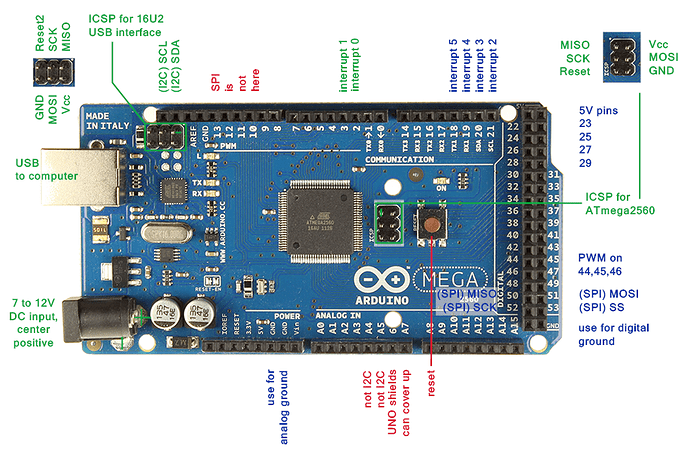
\includegraphics[width=0.7\textwidth]{resources/DomainAnalysis/HardwareComponents/arduino_mega_2560.png}%
}{%
    \fbox{\parbox{0.68\textwidth}{\centering\color{gray}\small
        [Photo pending --- save to resources/DomainAnalysis/HardwareComponents/arduino\_mega\_2560.png]}}%
}
\caption{Arduino Mega 2560 development board}
\label{fig:arduino_mega}
\end{figure}

\subsubsection{Push Button}

The circuit uses a standard momentary-action tactile push button. When pressed, it connects pin 7 of the microcontroller to GND, producing a LOW reading. The ATmega2560 internal pull-up is enabled, so no external resistor is required. Button bouncing is handled in software by the four-state FSM.

\begin{figure}[H]
\centering
\IfFileExists{resources/DomainAnalysis/HardwareComponents/pushbutton.png}{%
    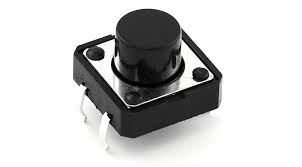
\includegraphics[width=0.35\textwidth]{resources/DomainAnalysis/HardwareComponents/pushbutton.png}%
}{%
    \fbox{\parbox{0.33\textwidth}{\centering\color{gray}\small
        [Photo pending --- save to resources/DomainAnalysis/HardwareComponents/pushbutton.png]}}%
}
\caption{Momentary tactile push button}
\label{fig:pushbutton}
\end{figure}

\subsubsection{LEDs and Current-Limiting Resistors}

Three 5\,mm LEDs --- green, red, and yellow --- provide the visual output. Each is driven through a 220\,$\Omega$ resistor, resulting in approximately 13.6\,mA forward current, within the ATmega2560 GPIO specifications.

\begin{figure}[H]
\centering
\IfFileExists{resources/DomainAnalysis/HardwareComponents/led.png}{%
    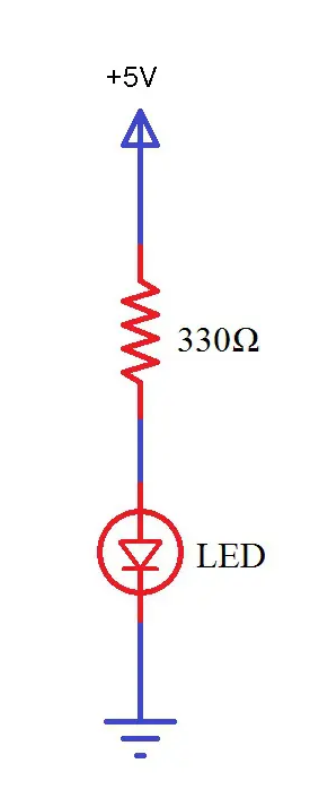
\includegraphics[width=0.4\textwidth]{resources/DomainAnalysis/HardwareComponents/led.png}%
}{%
    \fbox{\parbox{0.38\textwidth}{\centering\color{gray}\small
        [Photo pending --- save to resources/DomainAnalysis/HardwareComponents/led.png]}}%
}
\caption{Standard 5\,mm LED indicator component used for visual signaling}
\label{fig:led_component}
\end{figure}

\subsection{Software Components}

\subsubsection{PlatformIO Build System}

PlatformIO handles toolchain management, library resolution, and build configuration. Lab~2.2 is defined as an independent PlatformIO environment (\texttt{lab2\_2}) in \texttt{platformio.ini}, targeting the Arduino Mega 2560 with the FreeRTOS library as an external dependency via \texttt{lib\_deps = feilipu/FreeRTOS}.

\begin{figure}[H]
\centering
\IfFileExists{resources/DomainAnalysis/SoftwareComponents/platformio.png}{%
    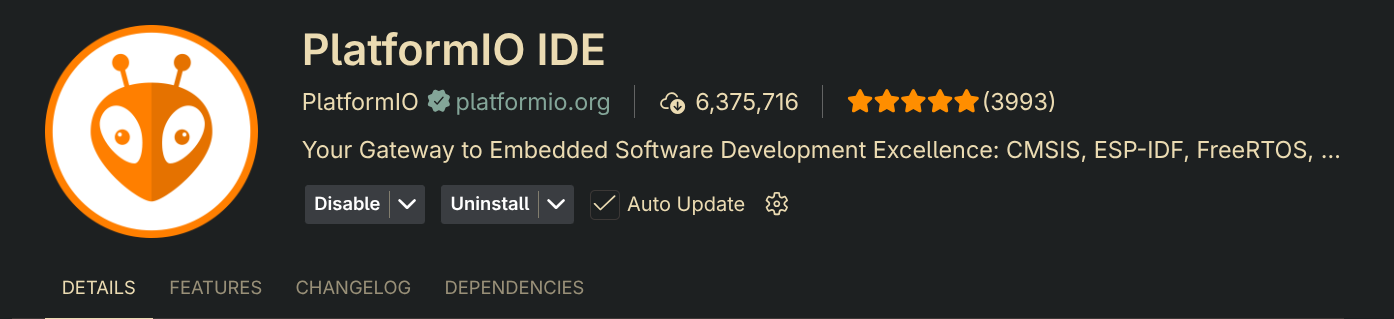
\includegraphics[width=0.75\textwidth]{resources/DomainAnalysis/SoftwareComponents/platformio.png}%
}{%
    \fbox{\parbox{0.73\textwidth}{\centering\color{gray}\small
        [Screenshot pending --- save to resources/DomainAnalysis/SoftwareComponents/platformio.png]}}%
}
\caption{PlatformIO workspace in VS Code showing the Lab 2.2 build environment}
\label{fig:platformio_env}
\end{figure}

\subsubsection{Wokwi Simulator}

The Wokwi VS Code plugin simulates the Arduino Mega 2560 circuit. The Lab~2.2 simulation uses the same \texttt{diagram.json} as Lab~2.1 (identical hardware), with \texttt{wokwi.toml} pointing to the \texttt{lab2\_2} firmware binary. Wokwi supports FreeRTOS-based firmware on AVR, enabling full functional testing of the preemptive scheduler, semaphore signaling, and mutex-protected data access.

\begin{figure}[H]
\centering
\IfFileExists{resources/DomainAnalysis/SoftwareComponents/wokwi.png}{%
    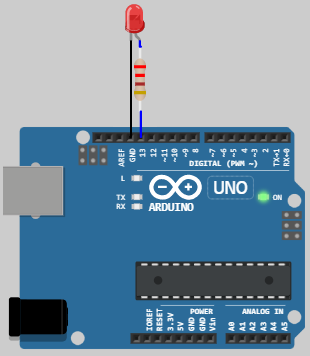
\includegraphics[width=0.6\textwidth]{resources/DomainAnalysis/SoftwareComponents/wokwi.png}%
}{%
    \fbox{\parbox{0.58\textwidth}{\centering\color{gray}\small
        [Screenshot pending --- save to resources/DomainAnalysis/SoftwareComponents/wokwi.png]}}%
}
\caption{Wokwi VS Code plugin used for circuit simulation and firmware testing}
\label{fig:wokwi_tool}
\end{figure}

\subsubsection{FreeRTOS Library (\texttt{feilipu/FreeRTOS})}

The \texttt{feilipu/FreeRTOS} library provides an Arduino-compatible port of FreeRTOS for AVR microcontrollers. It integrates with the Arduino framework by using Timer~3 (on Mega 2560) for the RTOS tick, leaving Timer~0 available for \texttt{millis()} and other Arduino timing functions. The library provides the full FreeRTOS API including \texttt{xTaskCreate()}, \texttt{vTaskDelay()}, \texttt{vTaskDelayUntil()}, binary semaphores, mutexes, and software timers. Default configuration uses a 1000\,Hz tick rate (1\,ms resolution), suitable for the 10\,ms polling period of Task~1.

\subsubsection{StdioSerial Library}

The \texttt{StdioSerial} library, originally developed in Laboratory Work 1.1, redirects AVR libc standard I/O streams to UART0, enabling \texttt{printf()} output over the USB serial link. It is reused without modification.

\subsection{Case Study: Automotive Embedded Systems with FreeRTOS}

FreeRTOS is the most widely deployed real-time operating system in the embedded industry, powering over 40 billion devices as of 2023. In the automotive domain, FreeRTOS is used in Electronic Control Units (ECUs) for body electronics, infotainment subsystems, and advanced driver assistance systems (ADAS). A typical body ECU monitors multiple button inputs (power windows, door locks, seat adjusters), classifies press durations (tap vs.\ hold), provides visual and haptic feedback, and reports diagnostics over a CAN bus at regular intervals --- a pattern directly analogous to the three-task architecture demonstrated in this laboratory.

The synchronization mechanisms employed in this lab --- binary semaphores for event notification and mutexes for data protection --- are the same primitives used in production automotive firmware. The priority inheritance feature of mutexes is particularly critical in automotive systems, where a missed deadline in a high-priority safety task (e.g., airbag deployment) due to priority inversion could have catastrophic consequences. The AUTOSAR OS specification mandates priority ceiling or priority inheritance protocols for exactly this reason.
